% abtex2-modelo-artigo.tex, v-1.9.2 laurocesar
% Copyright 2012-2014 by abnTeX2 group at http://abntex2.googlecode.com/ 
%

% ------------------------------------------------------------------------
% ------------------------------------------------------------------------
% abnTeX2: Modelo de Artigo Acadêmico em conformidade com
% ABNT NBR 6022:2003: Informação e documentação - Artigo em publicação 
% periódica científica impressa - Apresentação
% ------------------------------------------------------------------------
% ------------------------------------------------------------------------

\documentclass[
% -- opções da classe memoir --
article,			% indica que é um artigo acadêmico
11pt,				% tamanho da fonte
oneside,			% para impressão apenas no verso. Oposto a twoside
a4paper,			% tamanho do papel. 
% -- opções da classe abntex2 --
%chapter=TITLE,		% títulos de capítulos convertidos em letras maiúsculas
%section=TITLE,		% títulos de seções convertidos em letras maiúsculas
%subsection=TITLE,	% títulos de subseções convertidos em letras maiúsculas
%subsubsection=TITLE % títulos de subsubseções convertidos em letras maiúsculas
% -- opções do pacote babel --
english,			% idioma adicional para hifenização
brazil,				% o último idioma é o principal do documento
sumario=tradicional
]{abntex2}


% ---
% PACOTES
% ---

% ---
% Pacotes fundamentais 
% ---
\usepackage{lmodern}			% Usa a fonte Latin Modern
\usepackage[T1]{fontenc}		% Selecao de codigos de fonte.
\usepackage[utf8]{inputenc}		% Codificacao do documento (conversão automática dos acentos)
\usepackage{indentfirst}		% Indenta o primeiro parágrafo de cada seção.
\usepackage{nomencl} 			% Lista de simbolos
\usepackage{color}				% Controle das cores
\usepackage{graphicx}			% Inclusão de gráficos
\usepackage{float}
\usepackage{microtype} 			% para melhorias de justificação

% ---

% ---
% Pacotes adicionais, usados apenas no âmbito do Modelo Canônico do abnteX2
% ---
\usepackage{lipsum}				% para geração de dummy text
% ---

% ---
% Pacotes de citações
% ---
\usepackage[brazilian,hyperpageref]{backref}	 % Paginas com as citações na bibl
\usepackage[alf]{abntex2cite}	% Citações padrão ABNT
% ---

% ---
% Informações de dados para CAPA e FOLHA DE ROSTO
% ---
\titulo{Atividade VII}
\autor{ Rafael Gonçalves de Oliveira Viana}
\local{Brasil}
\data{2017}
% ---

% ---
% Configurações de aparência do PDF final

% alterando o aspecto da cor azul
\definecolor{blue}{RGB}{41,5,195}

% informações do PDF
\makeatletter
\hypersetup{
	%pagebackref=true,
	pdftitle={\@title}, 
	pdfauthor={\@author},
	pdfsubject={Artigo},
	pdfcreator={LaTeX with abnTeX2},
	pdfkeywords={abnt}{latex}{abntex}{abntex2}{atigo científico}, 
	colorlinks=true,       		% false: boxed links; true: colored links
	linkcolor=blue,          	% color of internal links
	citecolor=blue,        		% color of links to bibliography
	filecolor=magenta,      		% color of file links
	urlcolor=blue,
	bookmarksdepth=4
}
\makeatother
% --- 

% ---
% compila o indice
% ---
\makeindex
% ---

% ---
% Altera as margens padrões
% ---
\setlrmarginsandblock{3cm}{3cm}{*}
\setulmarginsandblock{3cm}{3cm}{*}
\checkandfixthelayout
% ---

% --- 
% Espaçamentos entre linhas e parágrafos 
% --- 

% O tamanho do parágrafo é dado por:
\setlength{\parindent}{1.3cm}

% Controle do espaçamento entre um parágrafo e outro:
\setlength{\parskip}{0.2cm}  % tente também \onelineskip

% Espaçamento simples
\SingleSpacing

% ----
% Início do documento
% ----
\begin{document}
	
	% Retira espaço extra obsoleto entre as frases.
	\frenchspacing 
	
	% ----------------------------------------------------------
	% ELEMENTOS PRÉ-TEXTUAIS
	% ----------------------------------------------------------
	
	%---
	%
	% Se desejar escrever o artigo em duas colunas, descomente a linha abaixo
	% e a linha com o texto ``FIM DE ARTIGO EM DUAS COLUNAS''.
	% \twocolumn[    		% INICIO DE ARTIGO EM DUAS COLUNAS
	%
	%---
	% página de titulo
	\maketitle
	\begin{enumerate}
		\item Procedure Alimenta Historico Forall
				\begin{verbatim}
					create or replace procedure Alimenta_Historico_Forall
					(ultima_turma in number, ultimo_aluno in number)
					is
					type tlista is table of number index by binary_integer;
					lista tlista;
					begin
					for j in 1..100 loop
					lista(j) := j;
					end loop;
					delete historico;
					for i in 1..ultima_turma loop
					forall j in 1..ultimo_aluno
					insert into historico (cod_turma, matricula) values (i,lista(j));
					end loop;
					commit;
					END;
				\end{verbatim}
				
				\begin{center}
					\begin{figure}[H]
						\centering
						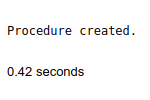
\includegraphics[scale=0.5]{./imagens/01.png}
						\caption{procedure criada.}
						\label{rota-1}
					\end{figure}
				\end{center}
		
			\item Procedure Alimenta Historico
				\begin{verbatim}
				create or replace procedure AlimentaHistorico
				(ultima_turma in number, ultimo_aluno in number)
				is
				begin
				delete historico; /* comentário: elimina registros atuais */
				for i in 1..ultima_turma loop
				for j in 1..ultimo_aluno loop
				insert into historico (cod_turma, matricula) values (i,j);
				end loop;
				end loop;
				commit;
				end;
				\end{verbatim}
				
				
				\begin{center}
					\begin{figure}[H]
						\centering
						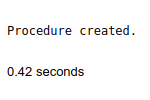
\includegraphics[scale=0.5]{./imagens/01.png}
						\caption{procedure criada.}
						\label{rota-1}
					\end{figure}
				\end{center}
		
			select object\_name from user\_objects where object\_type='PROCEDURE'
			
				\begin{center}
					\begin{figure}[H]
						\centering
						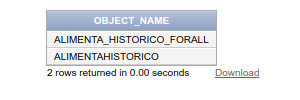
\includegraphics[scale=0.5]{./imagens/03.png}
						\caption{Select .}
						\label{rota-1}
					\end{figure}
				\end{center}
		
			\item Function Valor Em Dolar
					\begin{verbatim}
					create or replace function ValorEmDolar(reais in number, cotacao in number)
					return number
					is
					begin
					return reais/cotacao;
					end;
					\end{verbatim}
					
					\begin{center}
						\begin{figure}[H]
							\centering
							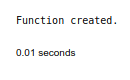
\includegraphics[scale=0.5]{./imagens/02.png}
							\caption{procedure criada.}
							\label{rota-1}
						\end{figure}
					\end{center}
				
				\item Function ValorEmDolar (segunda)
						\begin{verbatim}
					create or replace function ValorEmDolar
					(reais in number, cotacao in number)
					return number
					is
					begin
					return reais/cotacao;
					end;
						\end{verbatim}
						\begin{center}
							\begin{figure}[H]
								\centering
								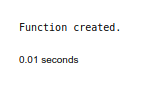
\includegraphics[scale=0.5]{./imagens/04.png}
								\caption{procedure criada.}
								\label{rota-1}
							\end{figure}
						\end{center}
						\begin{verbatim}
					Select nome_curso, preco "Em R$", ValorEmDolar(preco, 3.16) "Em
					US$" From cursos;
				    	\end{verbatim}
				   	\begin{center}
						   	\begin{figure}[H]
						   		\centering
						   		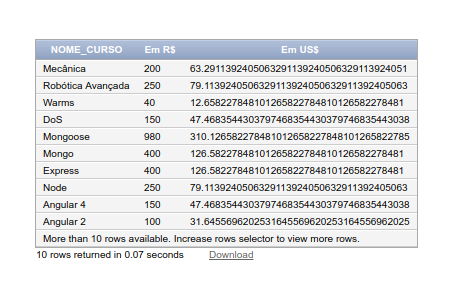
\includegraphics[scale=0.5]{./imagens/05.png}
						   		\caption{procedure criada.}
						   		\label{rota-1}
						   	\end{figure}
				   \end{center}
			   
			   Select object\_name from user\_objects where object\_type='FUNCTION';
			   
			    	\begin{center}
					   	\begin{figure}[H]
					   		\centering
					   		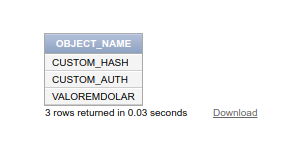
\includegraphics[scale=0.5]{./imagens/06.png}
					   		\caption{procedure criada.}
					   		\label{rota-1}
					   	\end{figure}
				   \end{center}
			 	\item Criar view vPessoas
			 \begin{verbatim}
			 create or replace function ValorEmDolar
			 (reais in number, cotacao in number)
			 return number
			 is
			 begin
			 return reais/cotacao;
			 end;
			 \end{verbatim}
			 \begin{center}
			 	\begin{figure}[H]
			 		\centering
			 		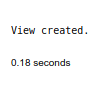
\includegraphics[scale=0.5]{./imagens/07.png}
			 		\caption{procedure criada.}
			 		\label{rota-1}
			 	\end{figure}
			 \end{center}
					
	\end{enumerate}				
			
\end{document}
